%%%%%%%%%%%%%%%%%%%%%%%%%%%%%%%%%%%%%%%%%%%%%%%%%%%%%%%%%%%%%%%%%%%%%%%%%%%%%%%
%%                                                                           %%
%%                             Trabajo indito                               %%
%%                                                                           %%
%%%%%%%%%%%%%%%%%%%%%%%%%%%%%%%%%%%%%%%%%%%%%%%%%%%%%%%%%%%%%%%%%%%%%%%%%%%%%%%

\cabecera{cap:faulttolerance}
                 {Fault tolerance}
\chapter{\textit{Fault tolerance}}
\label{cap:faulttolerance}
\cabecera{cap:Fault tolerance}
                 {Fault tolerance}

%%%%%%%%%%%%%%%%%%%%%%%%%%%%%%%%%%%%%%%%%%%%%%%%%%%%%%%%%%%%%%%%%%%%%%%%%%%%%%%

%\vfill
%\itshape
%En los problemas de clasificacin de patrones se busca minimizar el nmero de patrones mal clasificados (el error), sin embargo, en muchas aplicaciones reales hay que tener en cuenta por separado el error tipo I (falsos positivos) y el error tipo II (falsos negativos).
%Suele ser un problema complejo ya que un intento de minimizar uno de ellos, hace que el otro crezca.
%Es ms, en ocasiones uno de estos tipos de error puede ser ms importante que el otro, y se debe buscar un compromiso que minimice el ms importante de los dos.
%La medida estadstica ms utilizada, significancia estadstica, es una medida del error tipo I. Sin embargo, no ofrece garantas sobre el tipo II.

%A pesar de la importancia de los errores tipo II, la mayora de los mtodos de clasificacin slo tienen en cuenta el error de clasificacin global.
%En este trabajo se propone la optimizacin de ambos tipos de error de clasificacin utilizando un algoritmo multiobjetivo en el que cada tipo de error y el tamao de red son objetivos de la funcin de evaluacin (fitness).

%Se ha utilizado una versin modificada del mtodo G-Prop (diseo y optimizacin de perceptrones multicapa usando un algoritmo evolutivo) para optimizar simultneamente la estructura de la red neuronal y los errores tipo I y II.

%Debido a la carga computacional que supone la ejecucin de un algoritmo evolutivo para el diseo de redes neuronales, se propone la paralelizacin utilizando el modelo isla como forma de distribuir la carga en una red heterognea.
%\upshape
%\clearpage

%%%%%%%%%%%%%%%%%%%%%%%%%%%%%%%%%%%%%%%%%%%%%%%%%%%%%%%%%%%%%%%%%%%%%%%%%%%%%%%

%%%%%%%%%%%%%%%%%%%%%%%%%%%%%%%%%%%%%%%%%%%%%%%%%%%%%%%%%%%%%
P2P systems are large networks of volatile resources in which the collective dynamics of the peers are known as \emph{churn}. Therefore, addressing \emph{churn} in a P2P EA turns into a requirement of design rather than a mere study of fault tolerance.

Following the work by Stutzbach and Rejaie in \cite{Stutzbach06Understanding}, there are two main group-level properties of \emph{churn} which characterize the behaviour of all participating peers: The \emph{inter-arrival time} and the \emph{session length}, respectively, the time between two sessions and the time from the beginning to the end of a session.

In this study we have assumed that all nodes start at the same time with a certain \emph{session length}. The \emph{session length}  can be modeled randomly from a Weibull distribution using the following formula:

\begin{equation}\label{eq:weibull}
X = \lambda (-ln(U))^{\frac{1}{s}}
\end{equation}

\noindent
where $U$ is drawn from the uniform distribution, $s$ stands for the shape and $\lambda$ for the scale of the Weibull distribution. The analysis by Stutzbach and Rejaie exposes that the \emph{session length} of different P2P systems fit with a shape of $s \approx 0.40$ but the values of $\lambda$ differ. Additionally, the simulator driven experiments define the time unit as a simulator cycle which could apply for different time metrics in real time. Hence, we setup the following values for $\lambda=1,5,10,\infty$ depicted in Figure \ref{fig:ccdf}. It shows the complementary cumulative distribution functions (CCDF), representing the percentage of remaining nodes at each moment of the experiment for the different values of $\lambda$ (e.g. in the cycle 10, $\sim$8\% of the peers remain for $\lambda=1$ and $\sim$50\% for $\lambda=10$).


\begin{figure}[!htpb]
\centerline{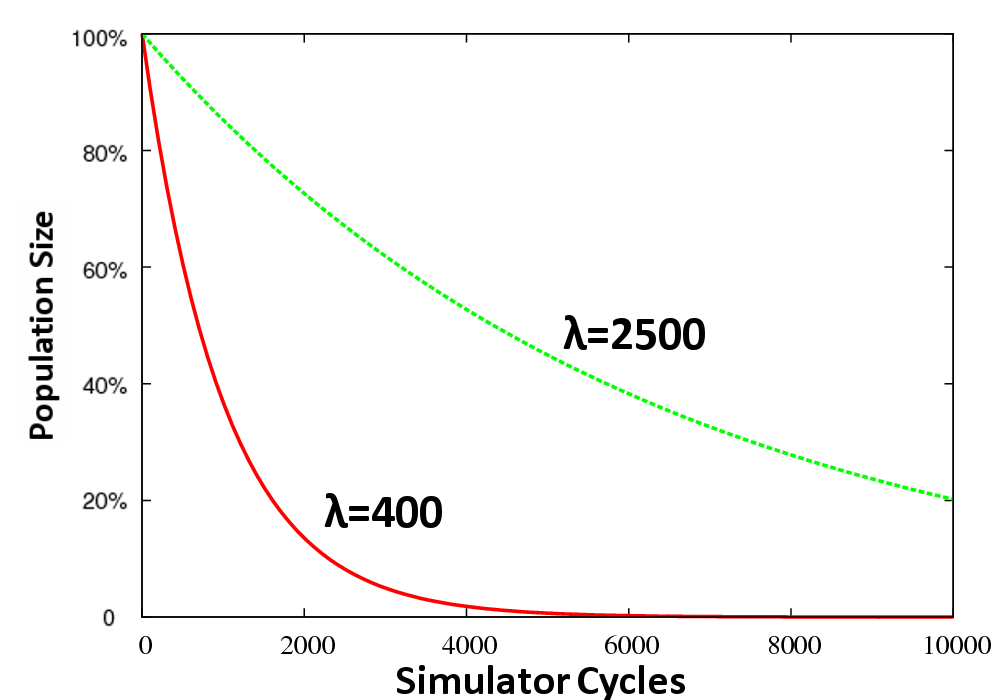
\includegraphics[width=3.8in]{ccdf}}
\caption{Complementary cumulative distribution functions}
\label{fig:ccdf}
\end{figure}

In spite of the initial assumption, the set of \emph{churn} scenarios allows a worst case analysis in which the system loses peers to zero. Once that a node leaves the experiment, it does not rejoin again (i.e. there is no \emph{inter-arrival}).

Under these conditions, several instances of the 4-trap function (i.e. $L= 8, 16, 32, 64$) have been used in order to assess the impact of \emph{churn} in the \emph{EvAg} model. Hence, there are three variables that affect the Success Rate (SR) of the algorithm: The size of the problem ($L$), which will conduct to a scalability analysis, the intensity of \emph{churn} ($\lambda$) and the population size ($P$). 

Any of the variables have the following influence on the SR if we assume a fixed value for the rest of them.
In the case of the problem instance, the bigger the size, the lower the SR. With respect to \emph{churn}, the more departures of nodes, the lower the SR. Finally, the bigger the population size, the higher the SR.

Being $\lambda$ and $L$ two independent variables under
the condition of obtaining a SR of 0.98, the population size can be
expressed as a function $f(\lambda,L)=P$ and empirically estimated using the bisection method. Furthermore, the runtime of the algorithm is also analysed as a function of the three variables $g(\lambda,L,P)$ since one of the goals in any distributed EA is to reduce the time for obtaining a solution.

Figure \ref{fig:populationsize} shows the scalability of the population size ($P$) as different curves of $L$, that is, $L$ scales and $\lambda$ remains fixed in $f(\lambda,L)=P$. The scalability of $f(\lambda,L)$ fits with a complexity order of $O(L^{(1.0,1.1)})$ in any of the scenarios. Hence, \emph{churn} does not  damage the scalability order (i.e. the curves are just shifted by a constant which is \emph{churn} dependent) and a reliable convergence can be guaranteed by ensuring enough resources. This fact points to the robustness of the Evolvable Agent model.


%%%%%%%%%%%%%%%%% 
\begin{figure}[!htpb]
\centerline{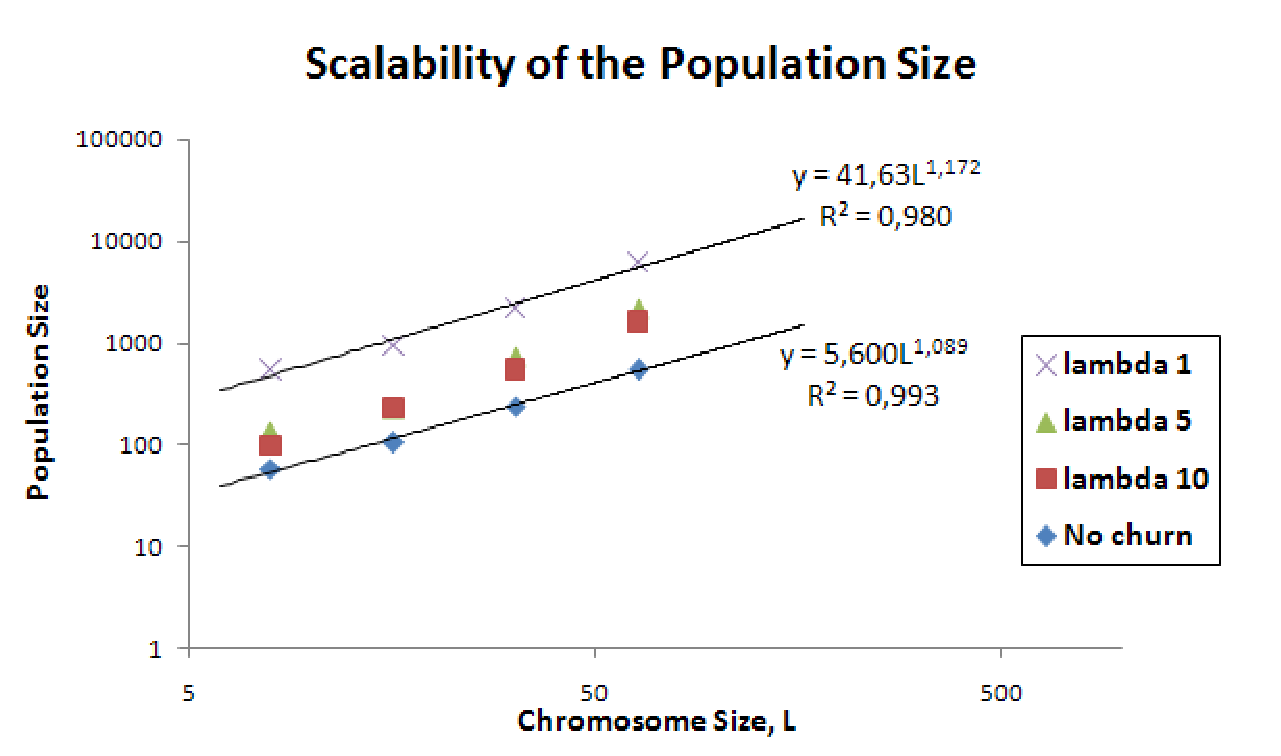
\includegraphics[width=3in]{churnpopulation}}
\caption{Scalability of the population size $f(\lambda,L)=P$ for the 4-trap in 4 scenarios of churn ($\lambda$)}
\label{fig:populationsize}
\end{figure}
%%%%%%%%%%%%%%%%% 

Additionally, Figure \ref{fig:responsetime} shows the runtime of
the algorithm $g(\lambda,L,P)$. $g$ is
independent from $\lambda$, with an order $O(L^{0.6})$. In
this case, \emph{churn} does not affect the
scalability (neither shifting the curves with a constant) and the
runtime is dependent on the problem instance
$L$. That means that we can expect the same runtime under any
\emph{churn} scenario if we ensure enough resources to satisfy the
0.98 of SR condition. Therefore, the algorithm is robust under \emph{churn}. 


%%%%%%%%%%%%%%%%% 
\begin{figure}[!htpb]
\centerline{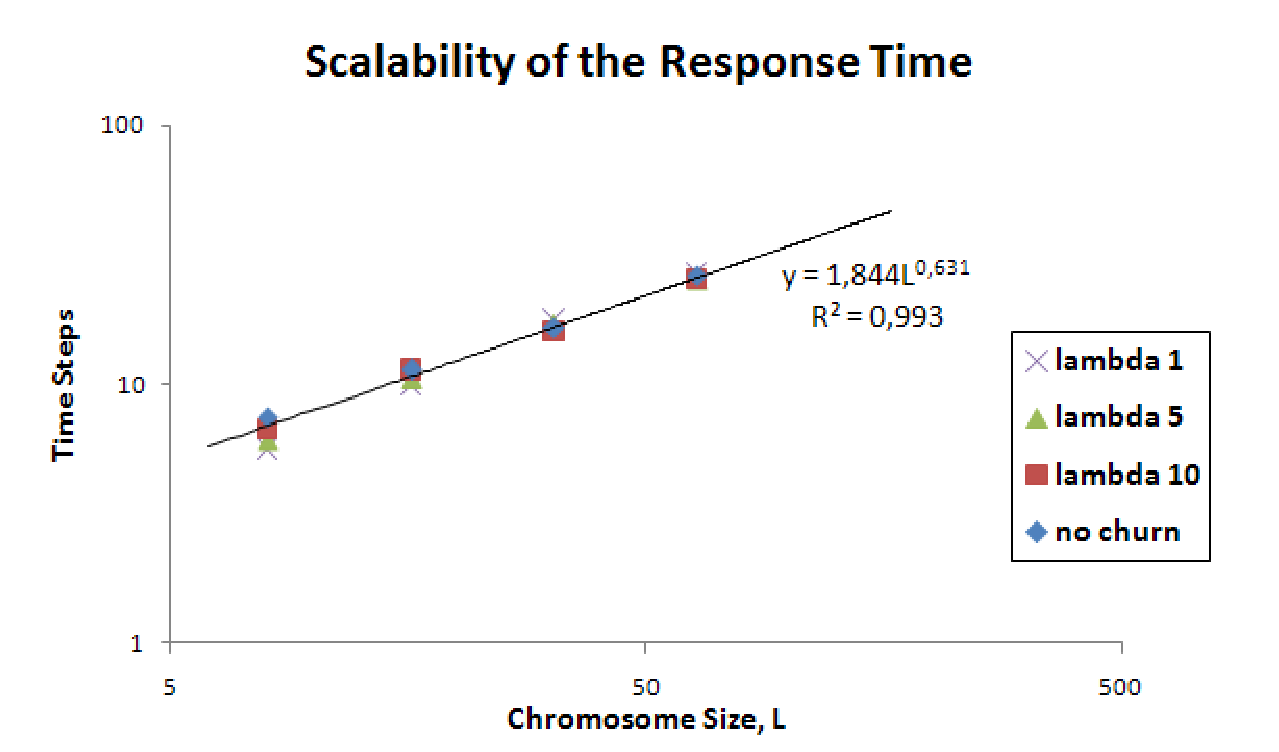
\includegraphics[width=3in]{churnresponse}}
\caption{Scalability of the runtime $g(\lambda,L,P)$ for the 4-trap in 4 scenarios of churn ($\lambda$) using $P$ estimated in $f(\lambda,L)$}
\label{fig:responsetime}
\end{figure}
%%%%%%%%%%%%%%%%% 

Figure \ref{fig:ccdfcycles} provides a better idea to the extent of these results.
 It represents the percentage of individuals of $P$ for which each experiment is expected to end. The effects of
\emph{churn} are more pernicious as the instances scale. In the worst case (i.e. $L=64$ and $\lambda=1$), the initial population ends with a $\sim$3\% of the individuals, still guaranteeing a SR of 0.98.


%%%%%%%%%%%%%%%%% 
\begin{figure}[!htpb]
\centerline{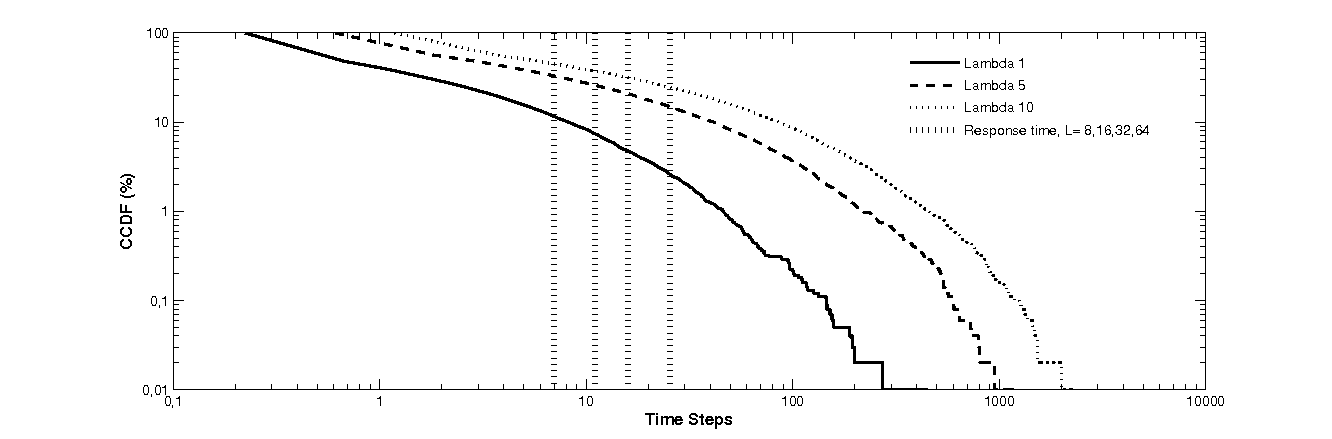
\includegraphics[width=3.5in]{ccdfcycles}}
\caption{Complementary cumulative distribution functions and average runtime}
\label{fig:ccdfcycles}
\end{figure}
%%%%%%%%%%%%%%%%% 
